\section{Tests and Results}

\subsection{Performance}

The processor can theoretically get up to a comfortable 73.573 MHz, according to Xilinx ISEs most accurate simulations (Post place and route).
Note that there is a 2ns difference in the minimum clock period between Post place and route and the XST - synthesize stage.
This is not that big of a surprise, as the data available to ISE is more accurate after the design has been mapped, placed and routed.
The obtained clock frequency is far above the required 24 MHz for the production simulation.

\begin{table}[h]
  \centering
  \begin{tabular}{lll}
    & Minimum period & Maximum frequency \\
    XST - Synthesize & 11.533ns &  86.705MHz \\
    Post place and route & 13.592ns &  73.573MHz \\
  \end{tabular}
  \caption{Critical paths and clock frequencies}
\end{table}

The system's critical path currently goes from Instruction memory, through the alu, out through the zero bit, and into the PC write condition.
If one wishes to attain a higher clock frequency, then the path has to be shortened.
This can happen either through the introduction of more flip-flops and control unit states, or by simplifying logic to avoid the problem alltogether.
It will be hard to remove this critical path in the design, so a much higher clock frequency might not be easily obtained.

Some alternate architectures were benchmarked, and one version with an additional fetch state between the current fetch and decode states was tested.
That architecture was able to run at roughly ~7 MHz faster than the one presented in this report.
Alas, 10\% clock frequency boost does not make up for the fact that all instructions would need an additional state (R-type instructions going from 4 to 5 states).

\subsection{Energy efficiency}

The multi cycle MIPS processor presented here is more power efficient than its single cycle counterparts.
Reuse of datapath elements during different parts of execution, as well as overlapping instruction execution provide area savings.
A short average-instruction execution time, as well as high maximum clock frequency (73.573MHz) reduces time to program completion and active power consumption.
The usage of dedicated FPGA resources such as block ram provides additional power savings over alternative implementations.

Generating post-place-and-route power data in Xilinx ISE give us a rough idea of what actual power consumption could look like \ref{tab:power-estimates}.
Xilinx considers these values inaccurate, but they can still be used to make ballpark estimates.
With these values, we could potentially calculate MIPS instructions for 5 full hours on a single coin cell battery (150 mah).

\begin{table}[h]
  \centering
  \begin{tabular}{llll}
    & Total & Dynamic & Quiescent \\
    Supply power (mW) & 29.60 & 5.58    & 24.02
  \end{tabular}
  \caption{Power estimates from Xilinx ISE}
  \label{tab:power-estimates}
\end{table}

Power constumption on an actual FPGA with the deployed programming was not tested.

\subsection{VHDL Testbenches}

% TODO: some parts of this might be better suited for solution or discussion?
All tests are written in VHDL and simulated in ISim.
Each component has been tested and verified with a separate testbench.
The system as a whole has also been tested with a separate testbech.
The mindset for the testbenches is to not only provide valuable testing to see if the compontents work,
but also make sure to give valueable feedback to the programmer.

The results of the tests are shown in table \ref{tab:tests}.

\begin{table}[ht+]
    \centering
    \begin{tabular}{|l|l|l|}
        \hline
        \textbf{Test name}            & \textbf{Pass?} & \textbf{Notes}            \\ \hline
        tb\_MIPSProcessor.vhd         & Passed         & Integrated machinery test \\ \hline
        tb\_alu.vhd                   & Passed         & Unit test                 \\ \hline
        tb\_control\_unit.vhd         & Passed         & Unit test                 \\ \hline
        tb\_instruction\_register.vhd & Passed         & Unit test                 \\ \hline
        tb\_mux.vhd                   & Passed         & Unit test                 \\ \hline
        tb\_mux\_4.vhd                & Passed         & Unit test                 \\ \hline
        tb\_pc.vhd                    & Passed         & Unit test                 \\ \hline
        tb\_registers.vhd             & Passed         & Unit test                 \\ \hline
        tb\_shift\_left\_2.vhd        & Passed         & Unit test                 \\ \hline
        tb\_sign\_extend.vhd          & Passed         & Unit test                 \\ \hline
    \end{tabular}
    \caption{Tests being performed on the processor}
    \label{tab:tests}
\end{table}

\subsubsection{Top level testbench}

A top-level testbench was provided, so that we could confirm that the processor worked as the exercise had intended.
It consists of a test program which is loaded into instruction memory, as well as some initial data.

Here follows several screenshots from the test simulation, showing how different instruction types are executed in the implemented processor.
They show what state the processor is currently in, as well as the currently executing instruction.
The complete run of the toplevel testbench can be seen in Figure \ref{fig:tb_toplevel} in Appendix A.

\begin{figure}[ht!]
    \begin{center}
    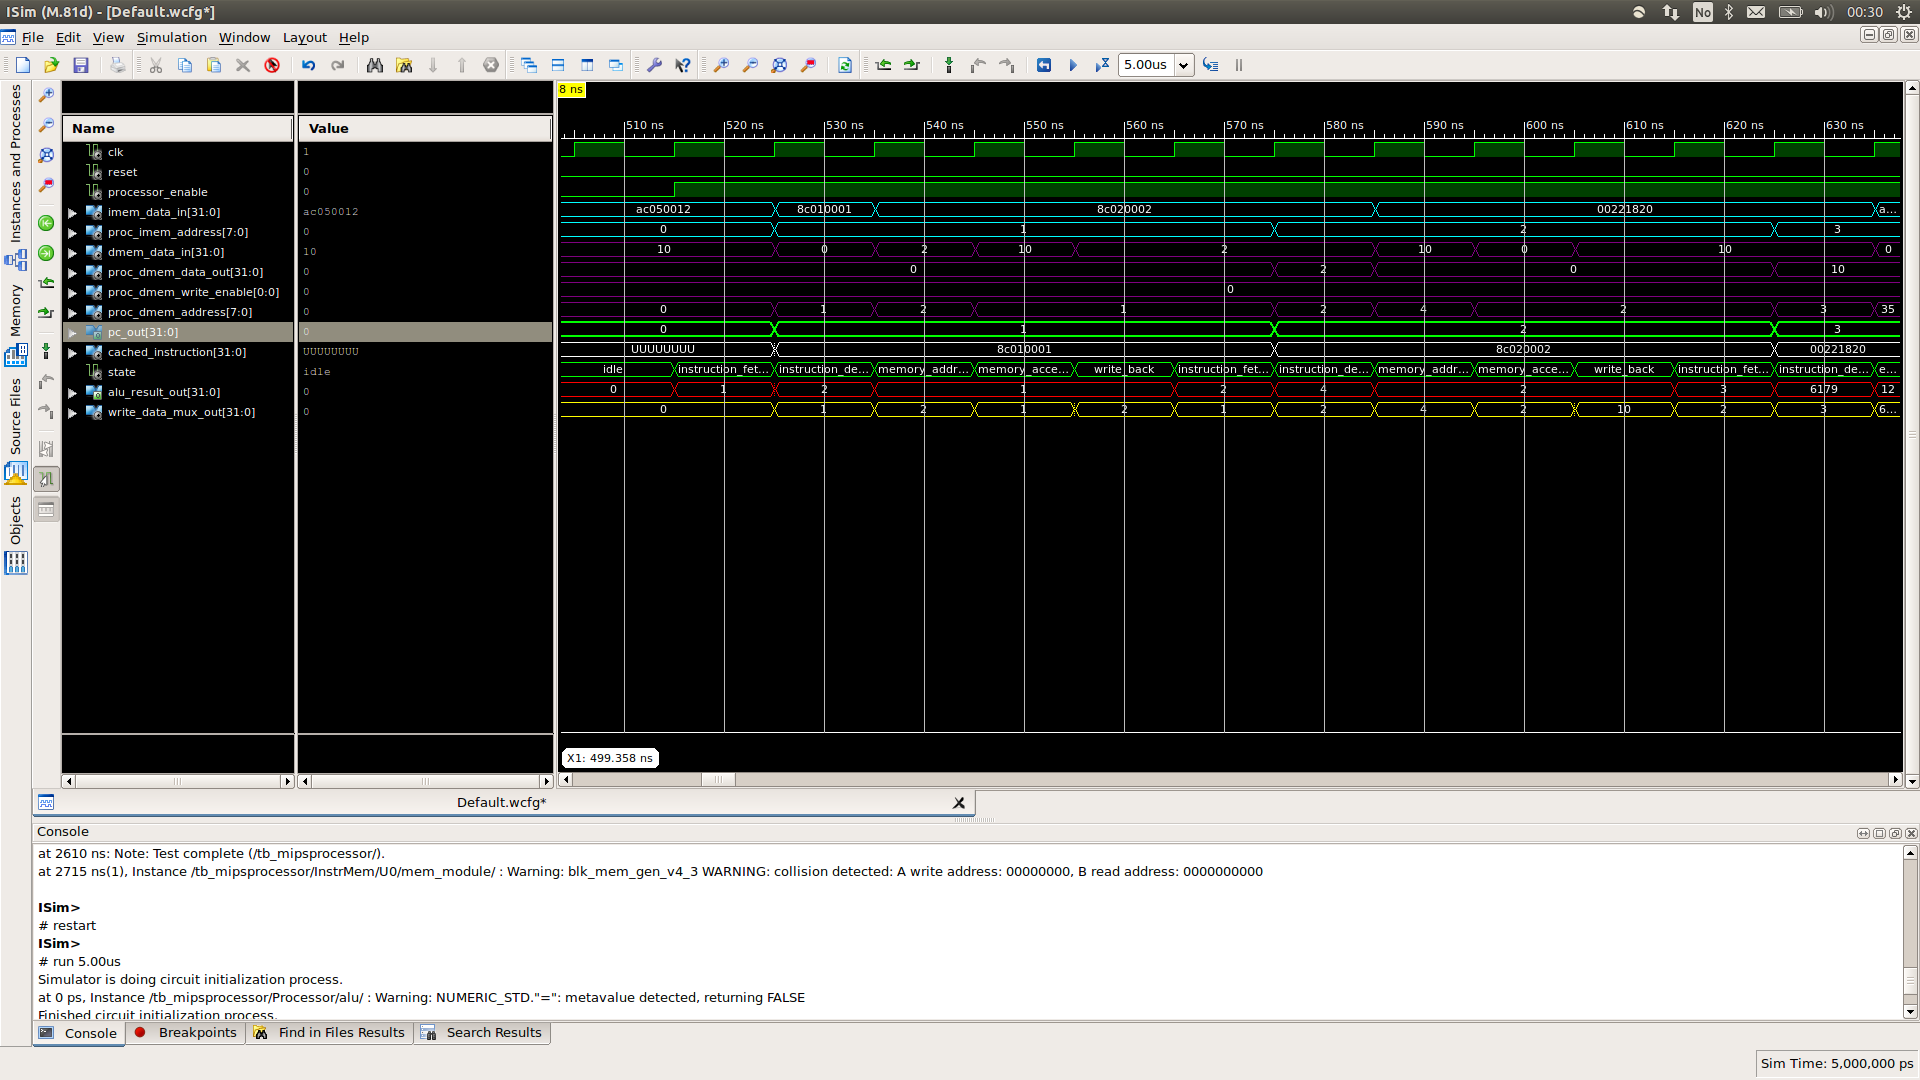
\includegraphics[width=\textwidth]{assets/isim/memory_read_cycle.png}
    \caption{Snapshot of the top level testbench when executing a load instruction}
    \label{fig:memory_read_cycle}
    \end{center}
\end{figure}

\begin{figure}[ht!]
    \begin{center}
    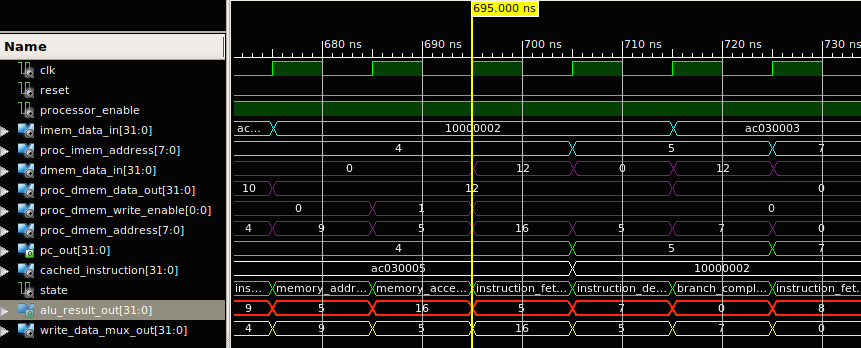
\includegraphics[width=\textwidth]{assets/isim/branch_completion_cycle.png}
    \caption{Snapshot of the top level testbench when running a branch instruction}
    \label{fig:branch_completion_cycle}
    \end{center}
\end{figure}

\begin{figure}[ht!]
    \begin{center}
    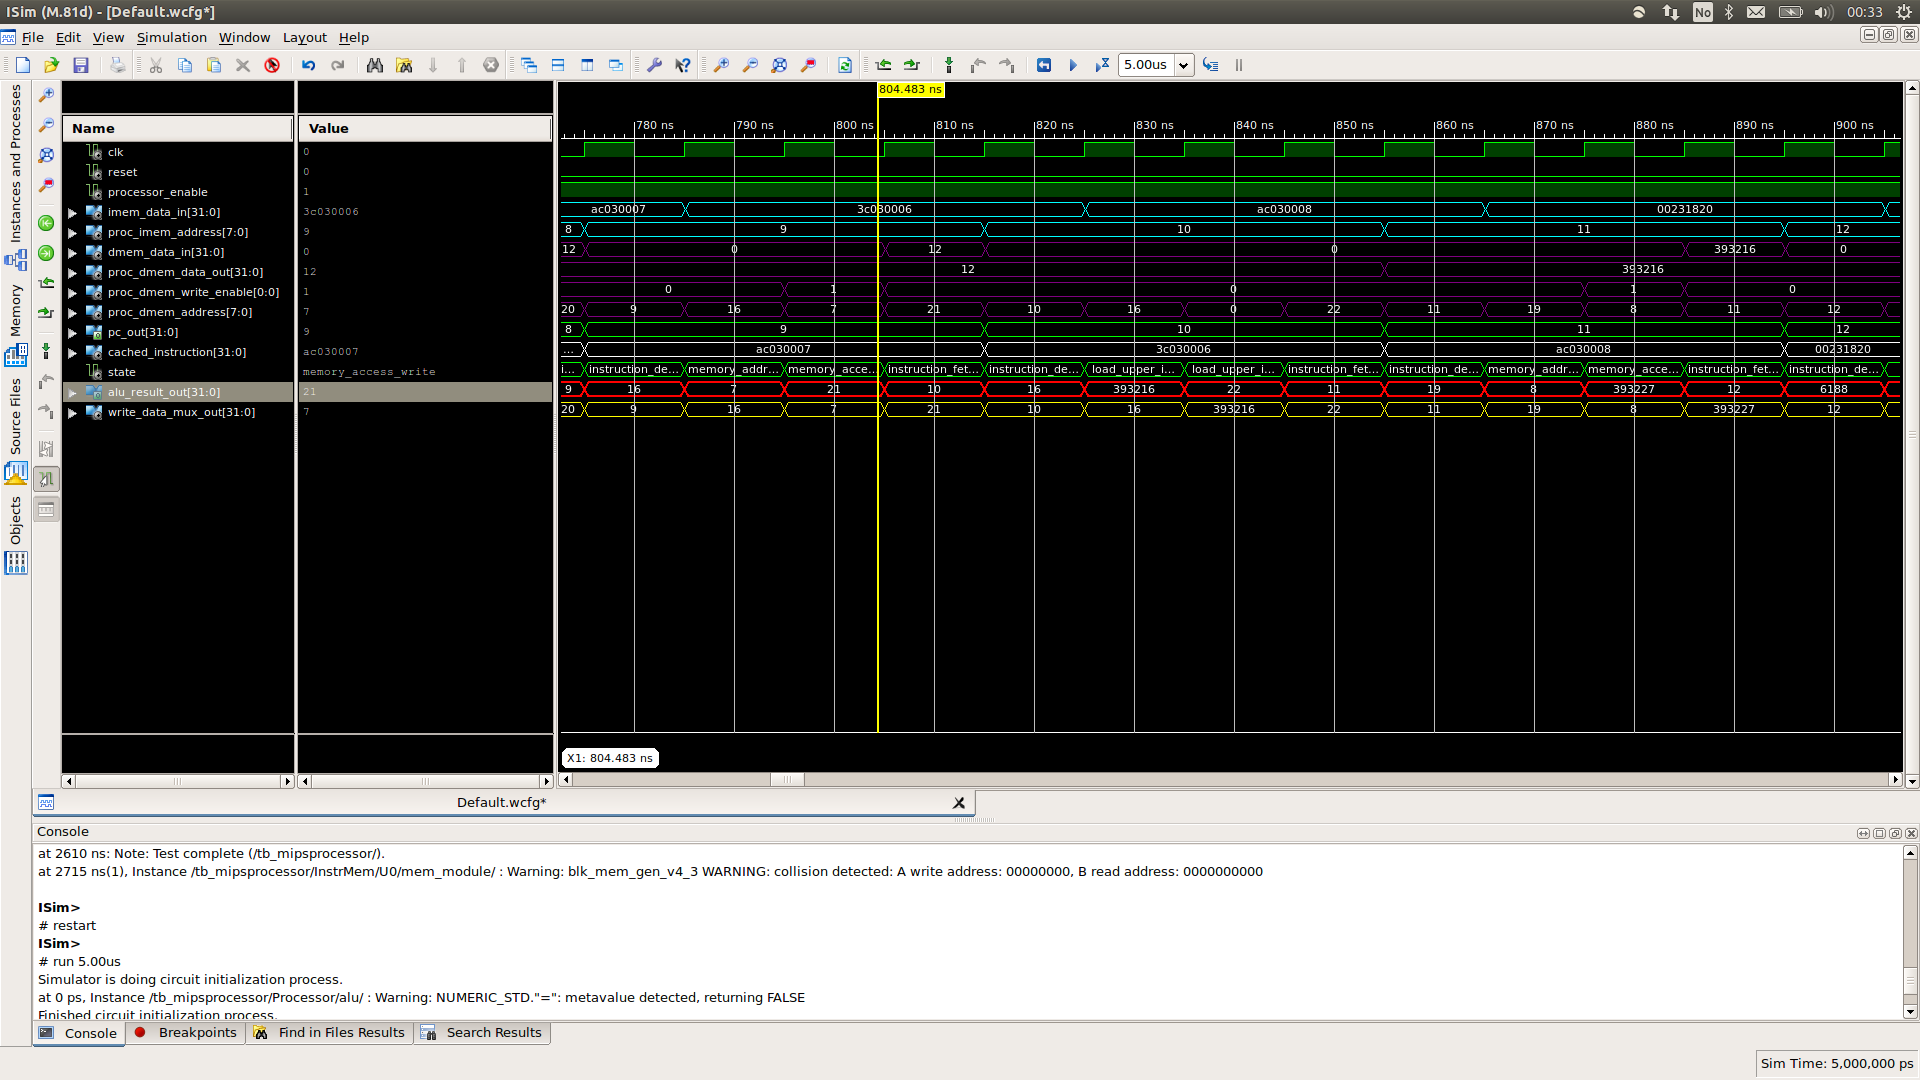
\includegraphics[width=\textwidth]{assets/isim/load_upper_cycle.png}
    \caption{Execution of a load immediate, where the value 393216 is stored in register 3}
    \label{fig:load_upper_cycle}
    \end{center}
\end{figure}

\begin{figure}[ht!]
    \begin{center}
    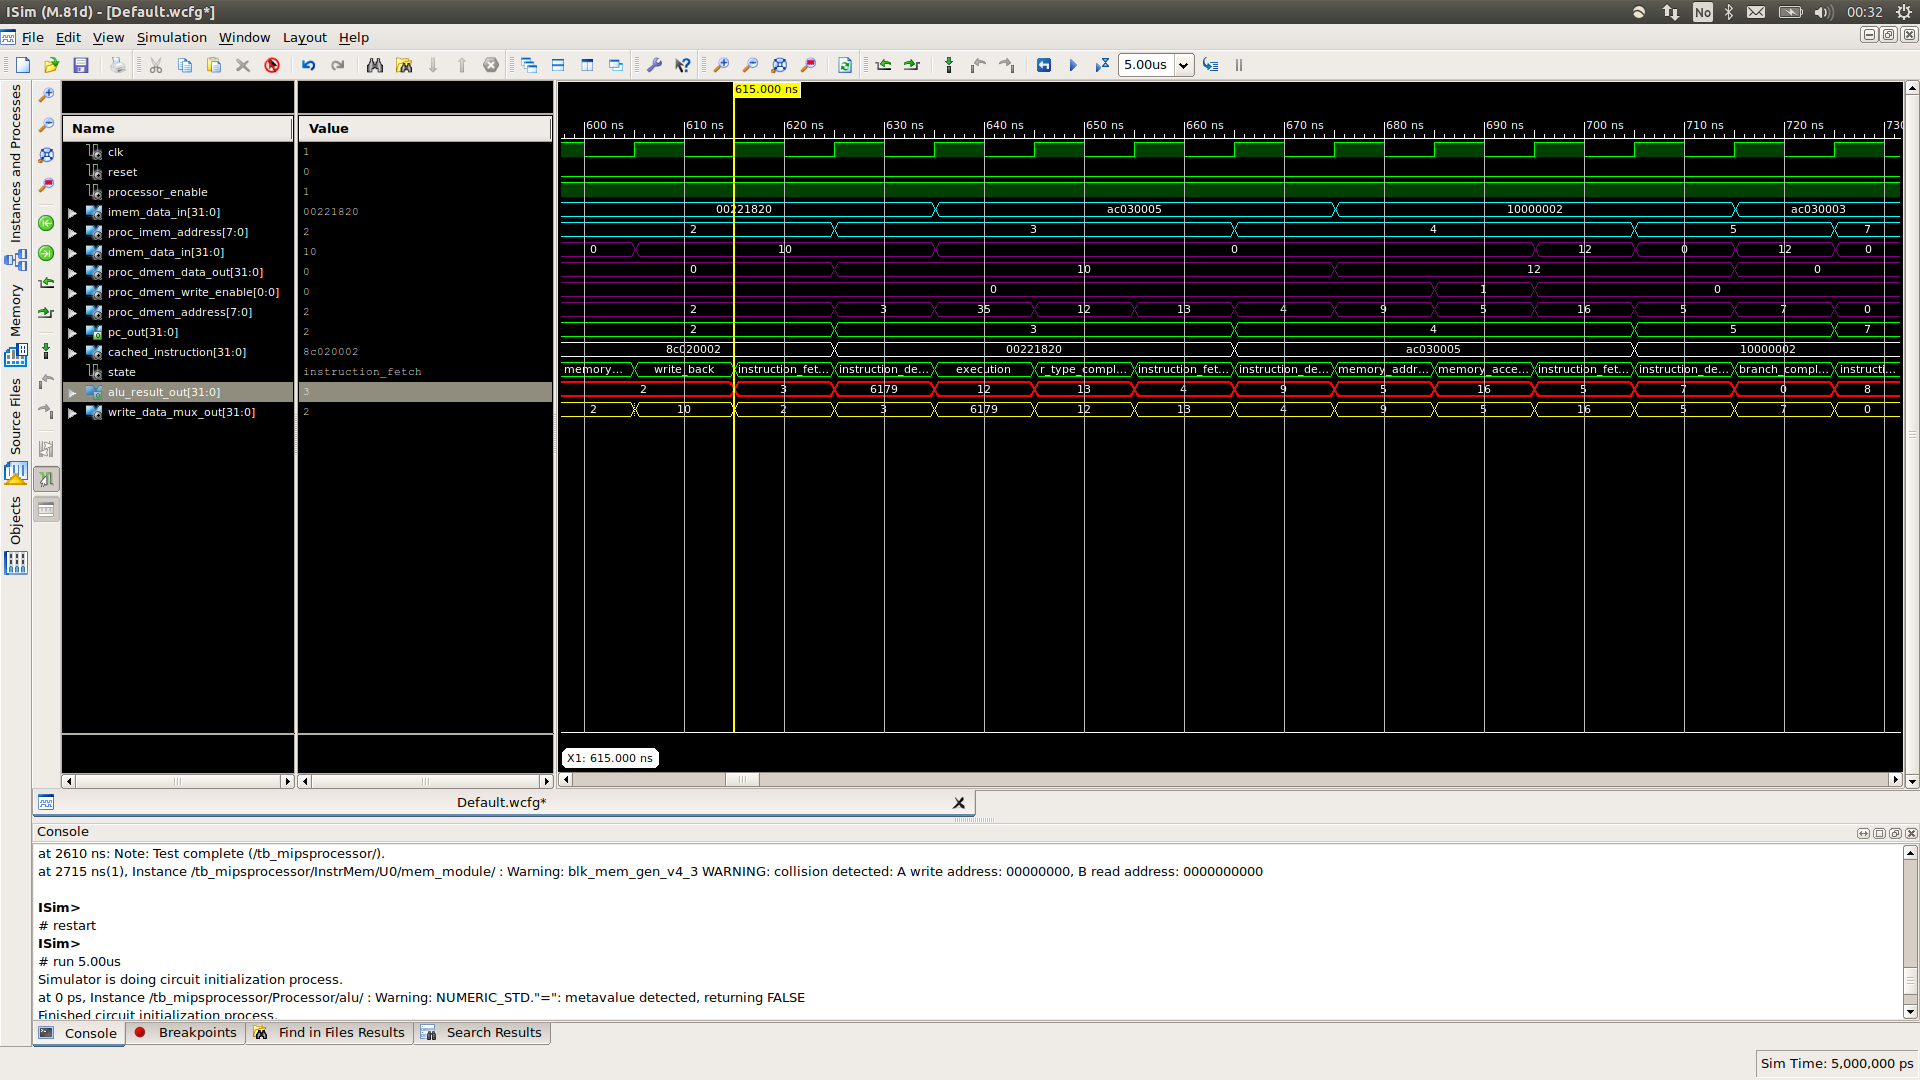
\includegraphics[width=\textwidth]{assets/isim/r_type_cycle.png}
    \caption{An r-type instruction with ALU op set to ADD}
    \label{fig:r_type_cycle}
    \end{center}
\end{figure}

\clearpage

\subsection{Testing on hardware}

% TODO: a series of steps need to be taken?
When testing on the actual hardware, a series of steps needs to be taken.
These steps are illustrated in figure \ref{fig:testing_on_fpga}.

Firstly a .bit file must be generated form Xilinx.
This file is then uploaded to the FPGA via the hostcomm utility.
Afterwards a simple program is made, or taken from the testbench for the processor.

The endianness of the hostcomm utility \cite{hostcomm} is different from the testbench.
Because of that a simple translator was written in python to change
the endianness of the sample program \cite{endian-change}.
This program made it possible to paste its output straight into hostcomm.

With the program in the hostcomm utility, one can upload it to the fpga.
A button in hostcomm runs the program and afterwards there is a possibility to read form the FPGA memory.

The content of the FPGA memory is then verified against expected output manually.

\begin{figure}[ht!]
    \begin{center}
        \subfigure[Generate .bit file from Xilinx]{%
            \label{fig:generate_fpga}
            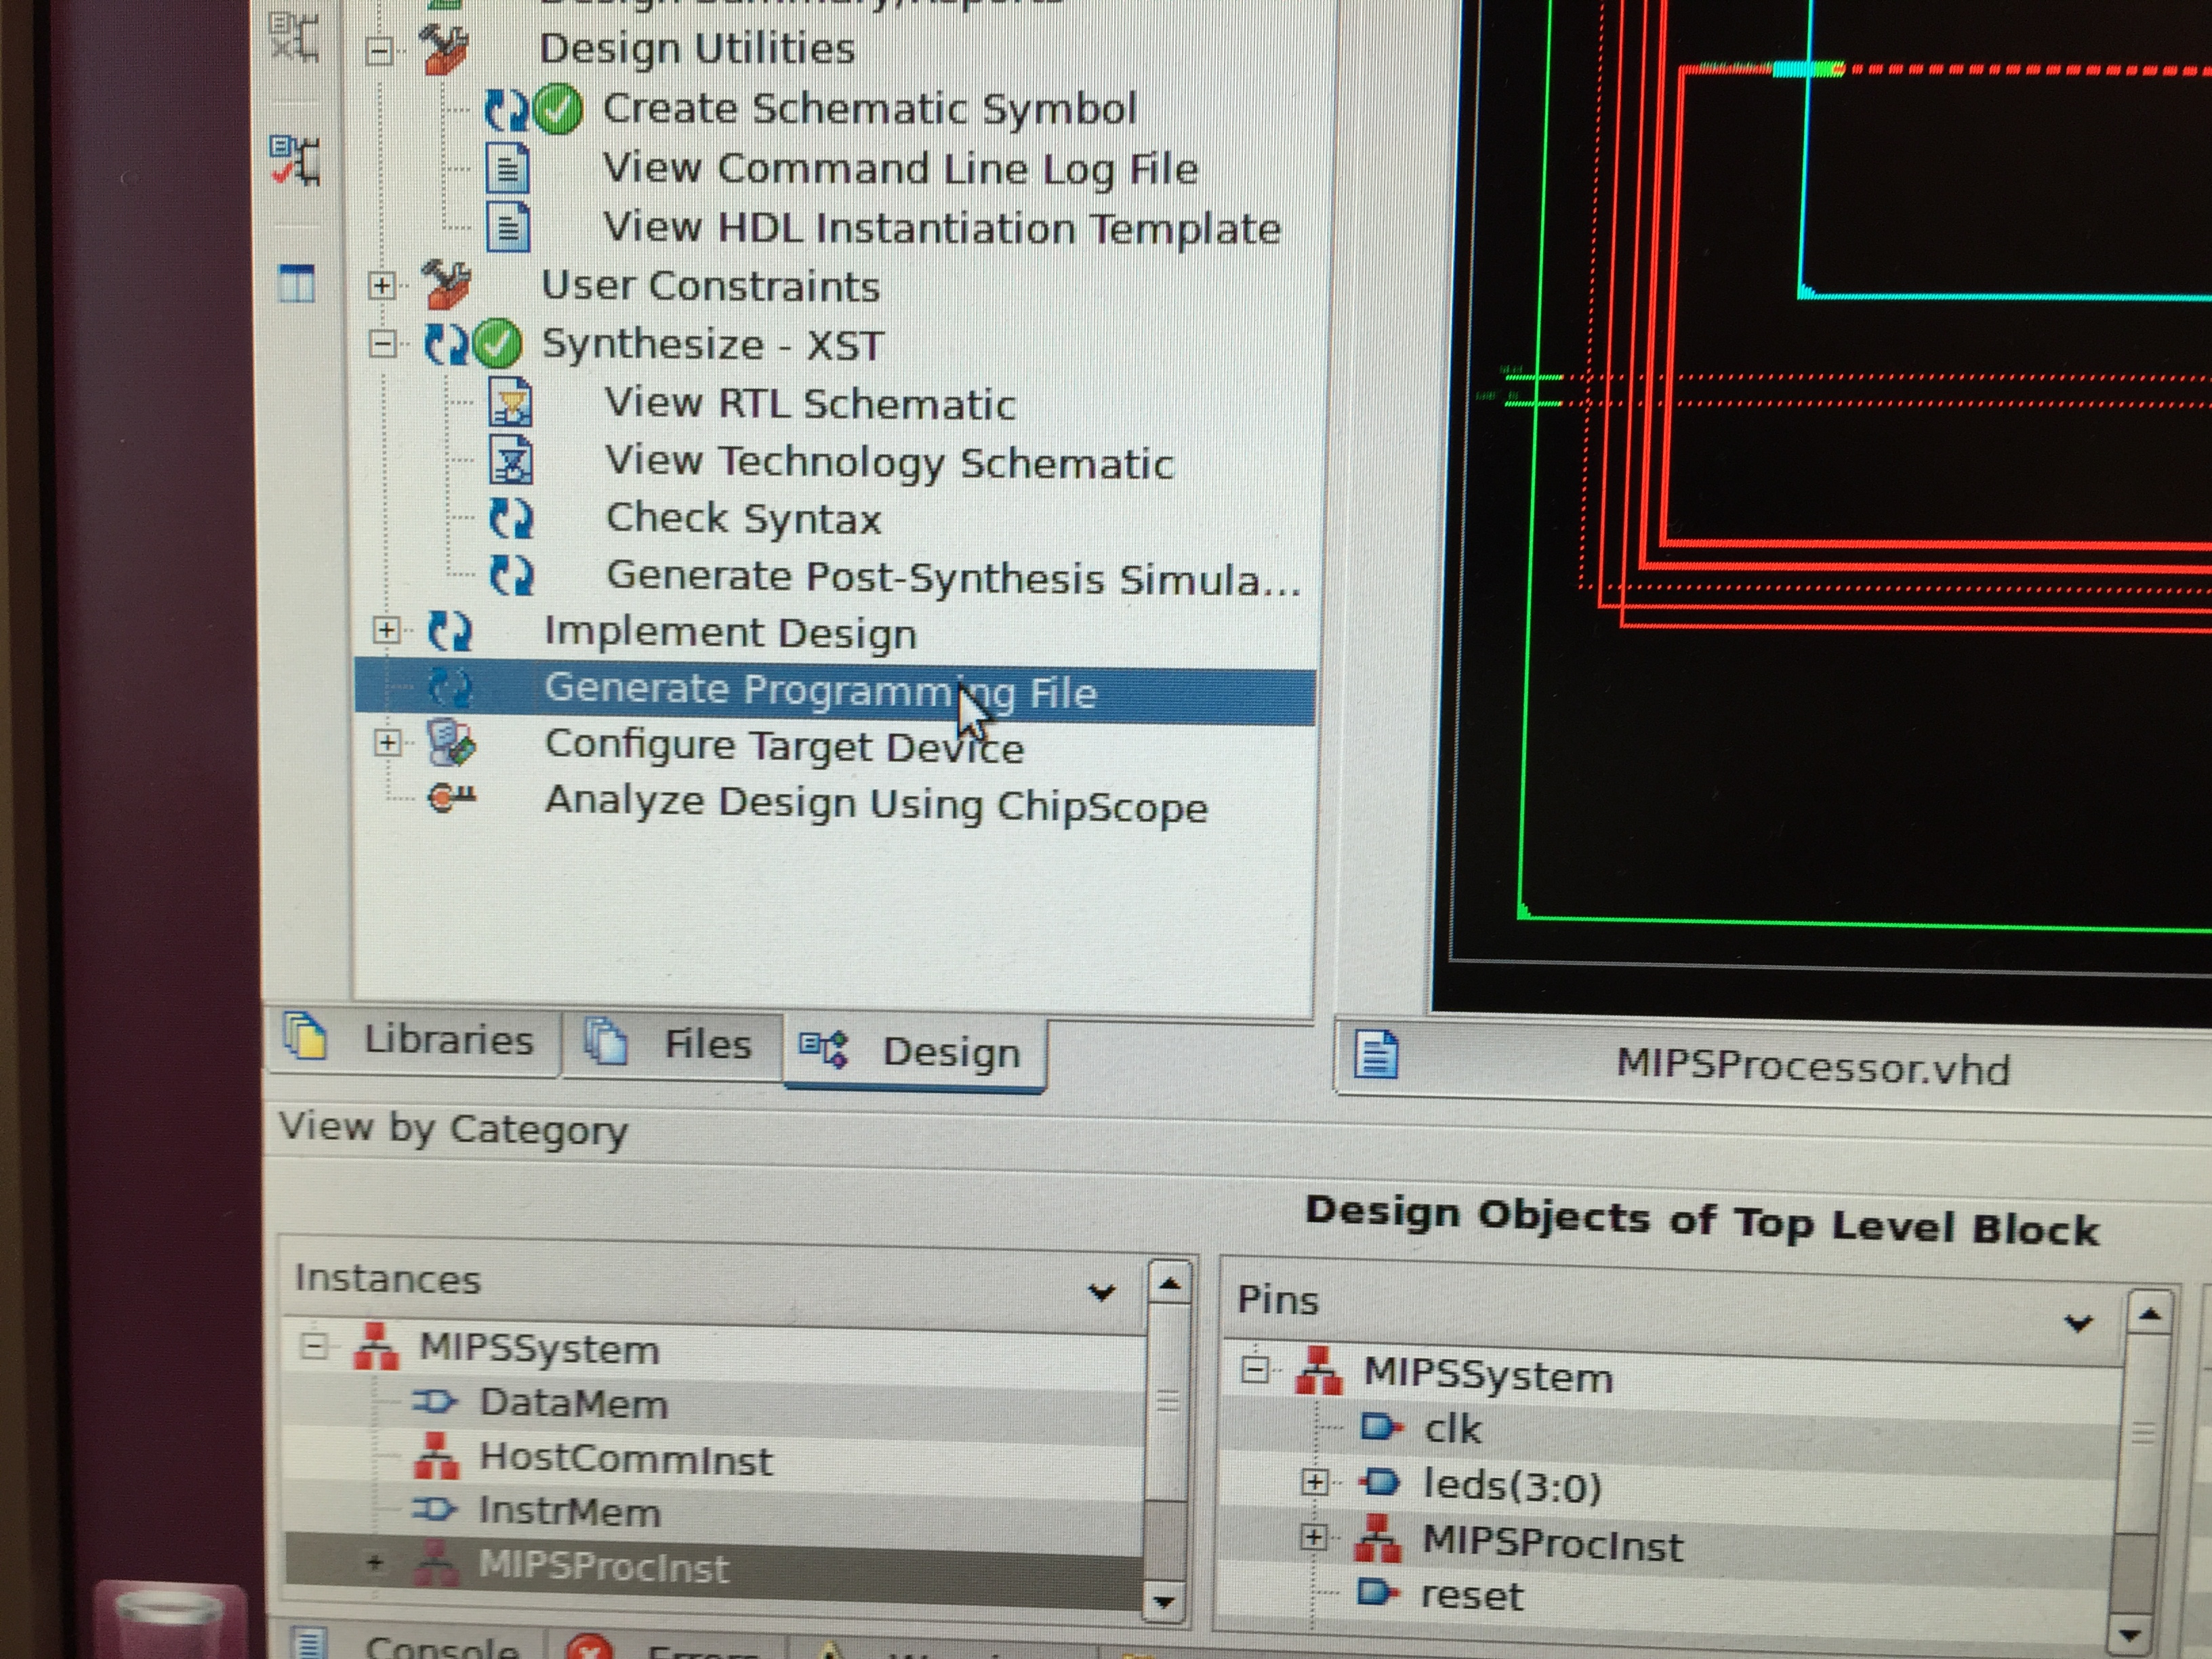
\includegraphics[width=0.4\textwidth]{assets/testing_on_fpga/generate_programming_file.JPG}
        }%
        \subfigure[Upload .bit file to the FPGA]{%
            \label{fig:processor_upload_fpga}
            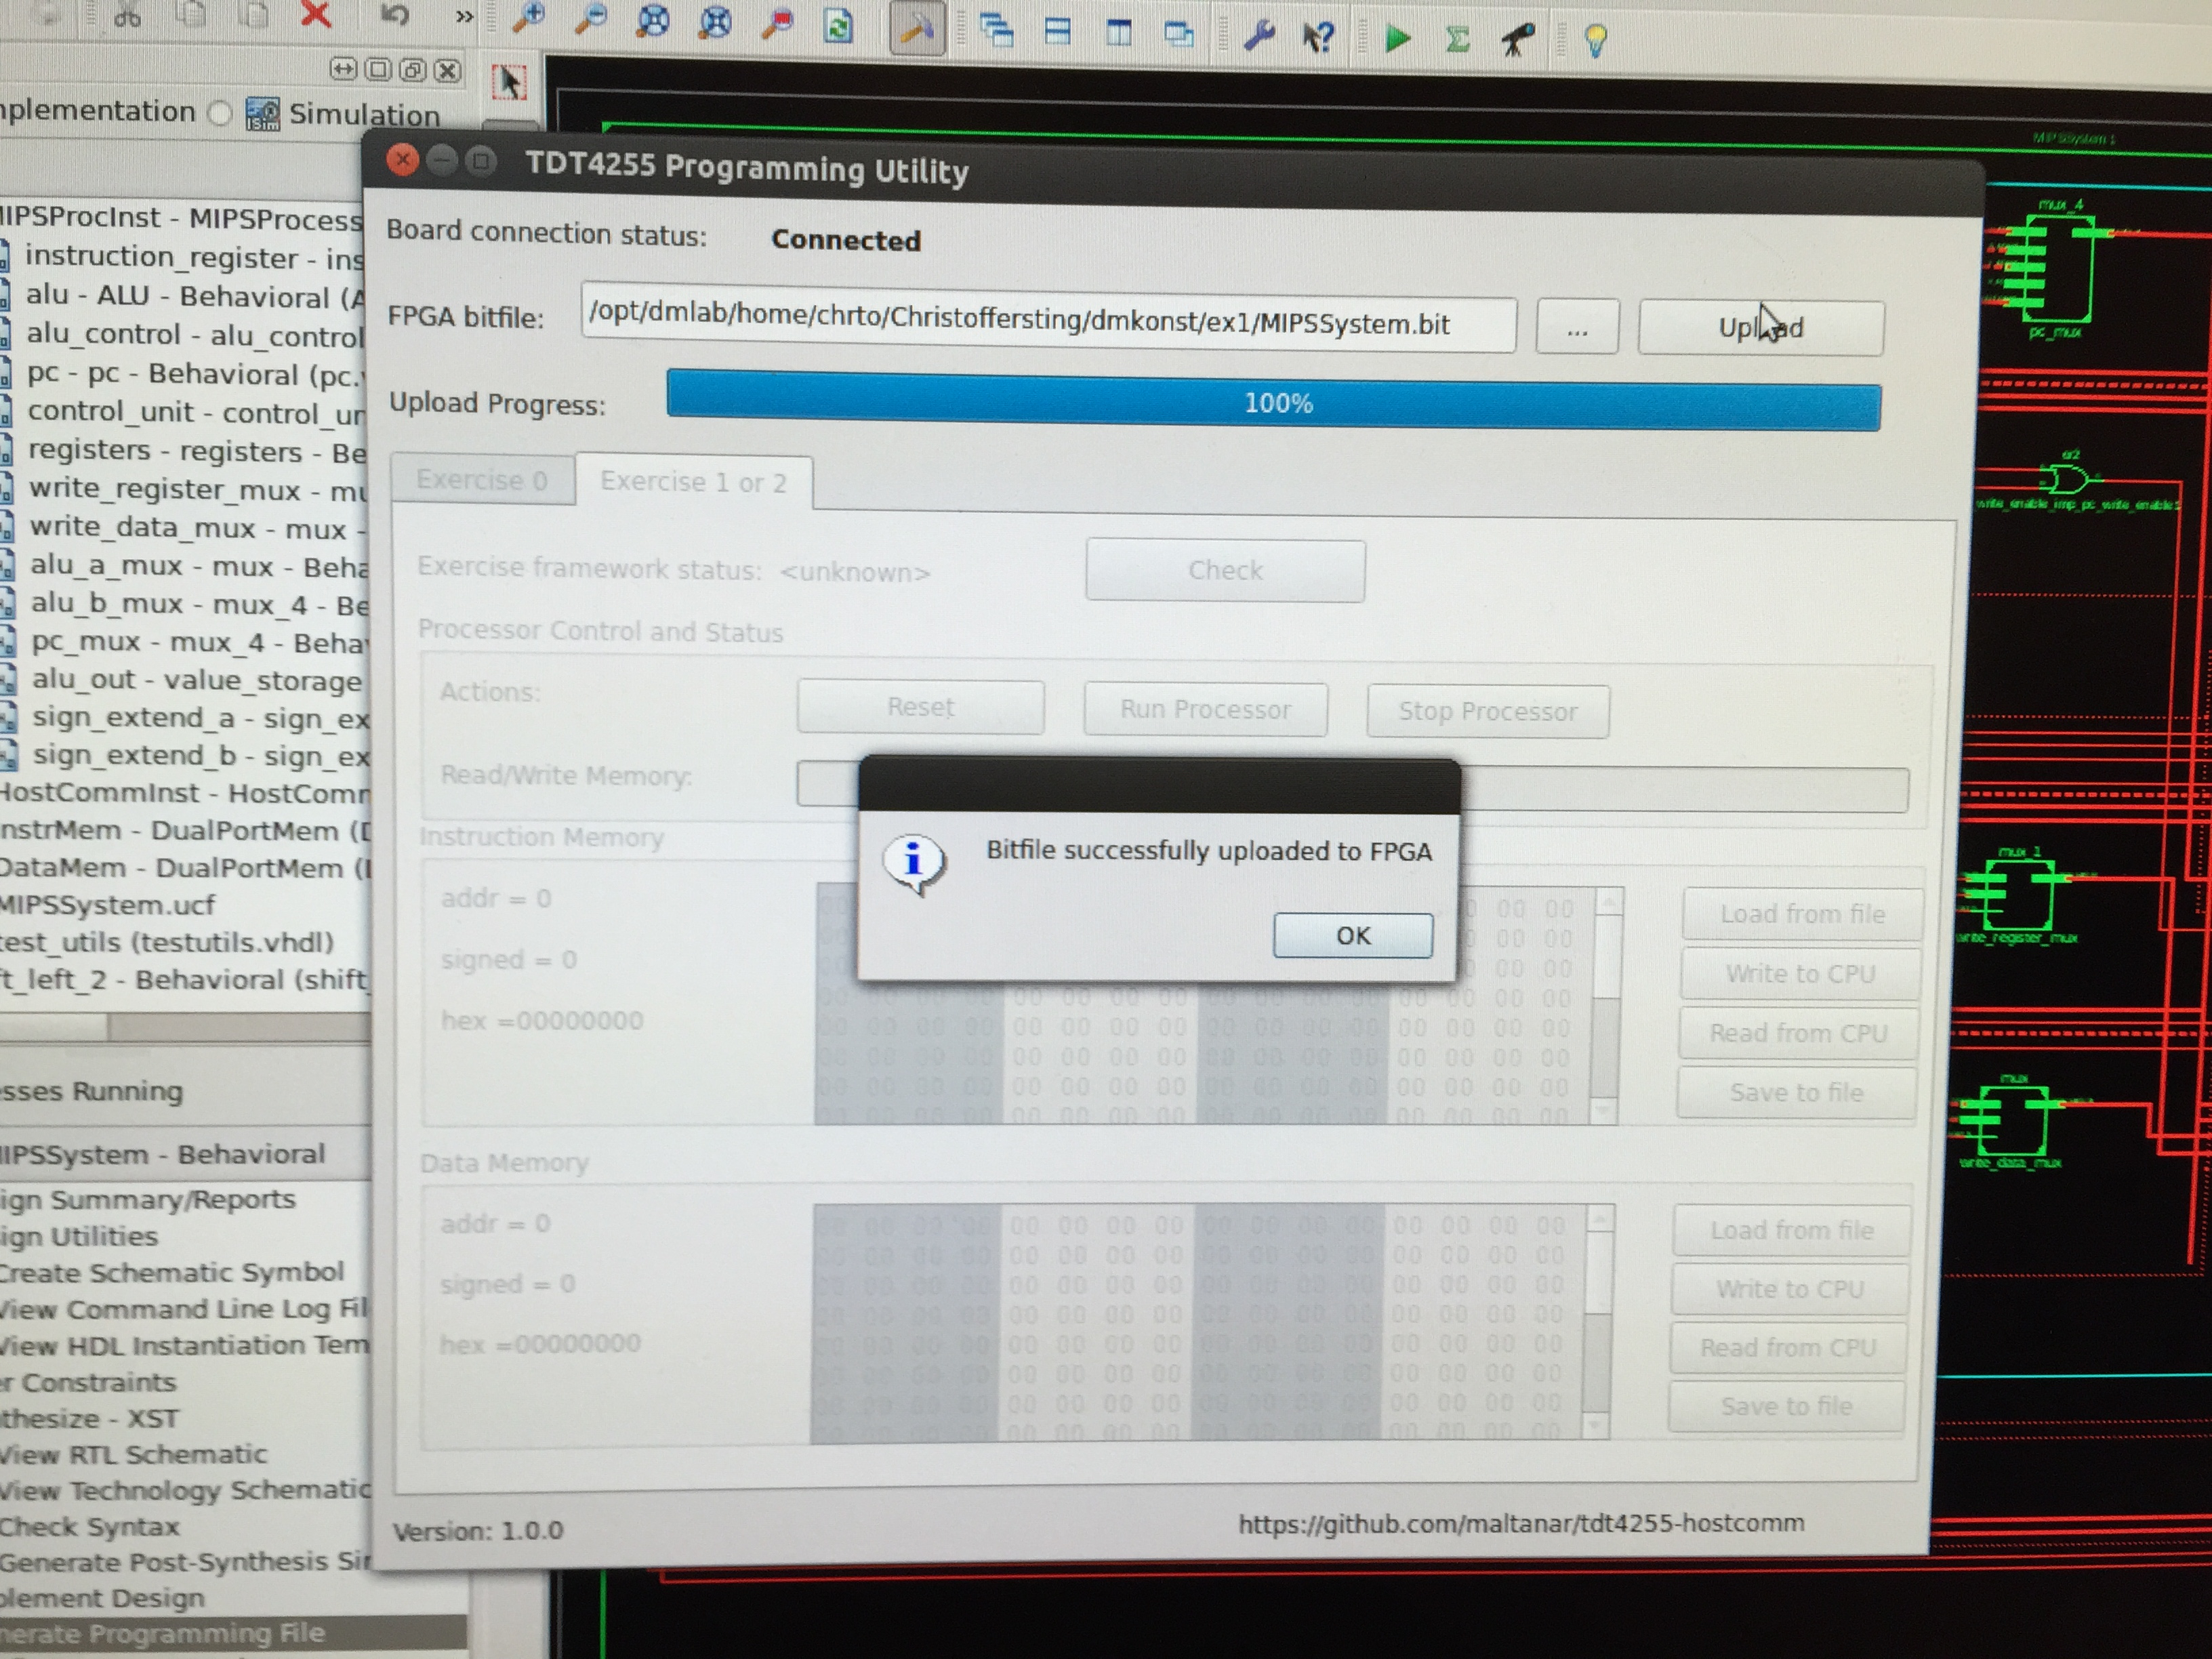
\includegraphics[width=0.4\textwidth]{assets/testing_on_fpga/uploaded_successfully.JPG}
        }\\ %  ------- End of the first row ----------------------%
        \subfigure[Change endianness]{%
            \label{fig:endinanness_fpga}
            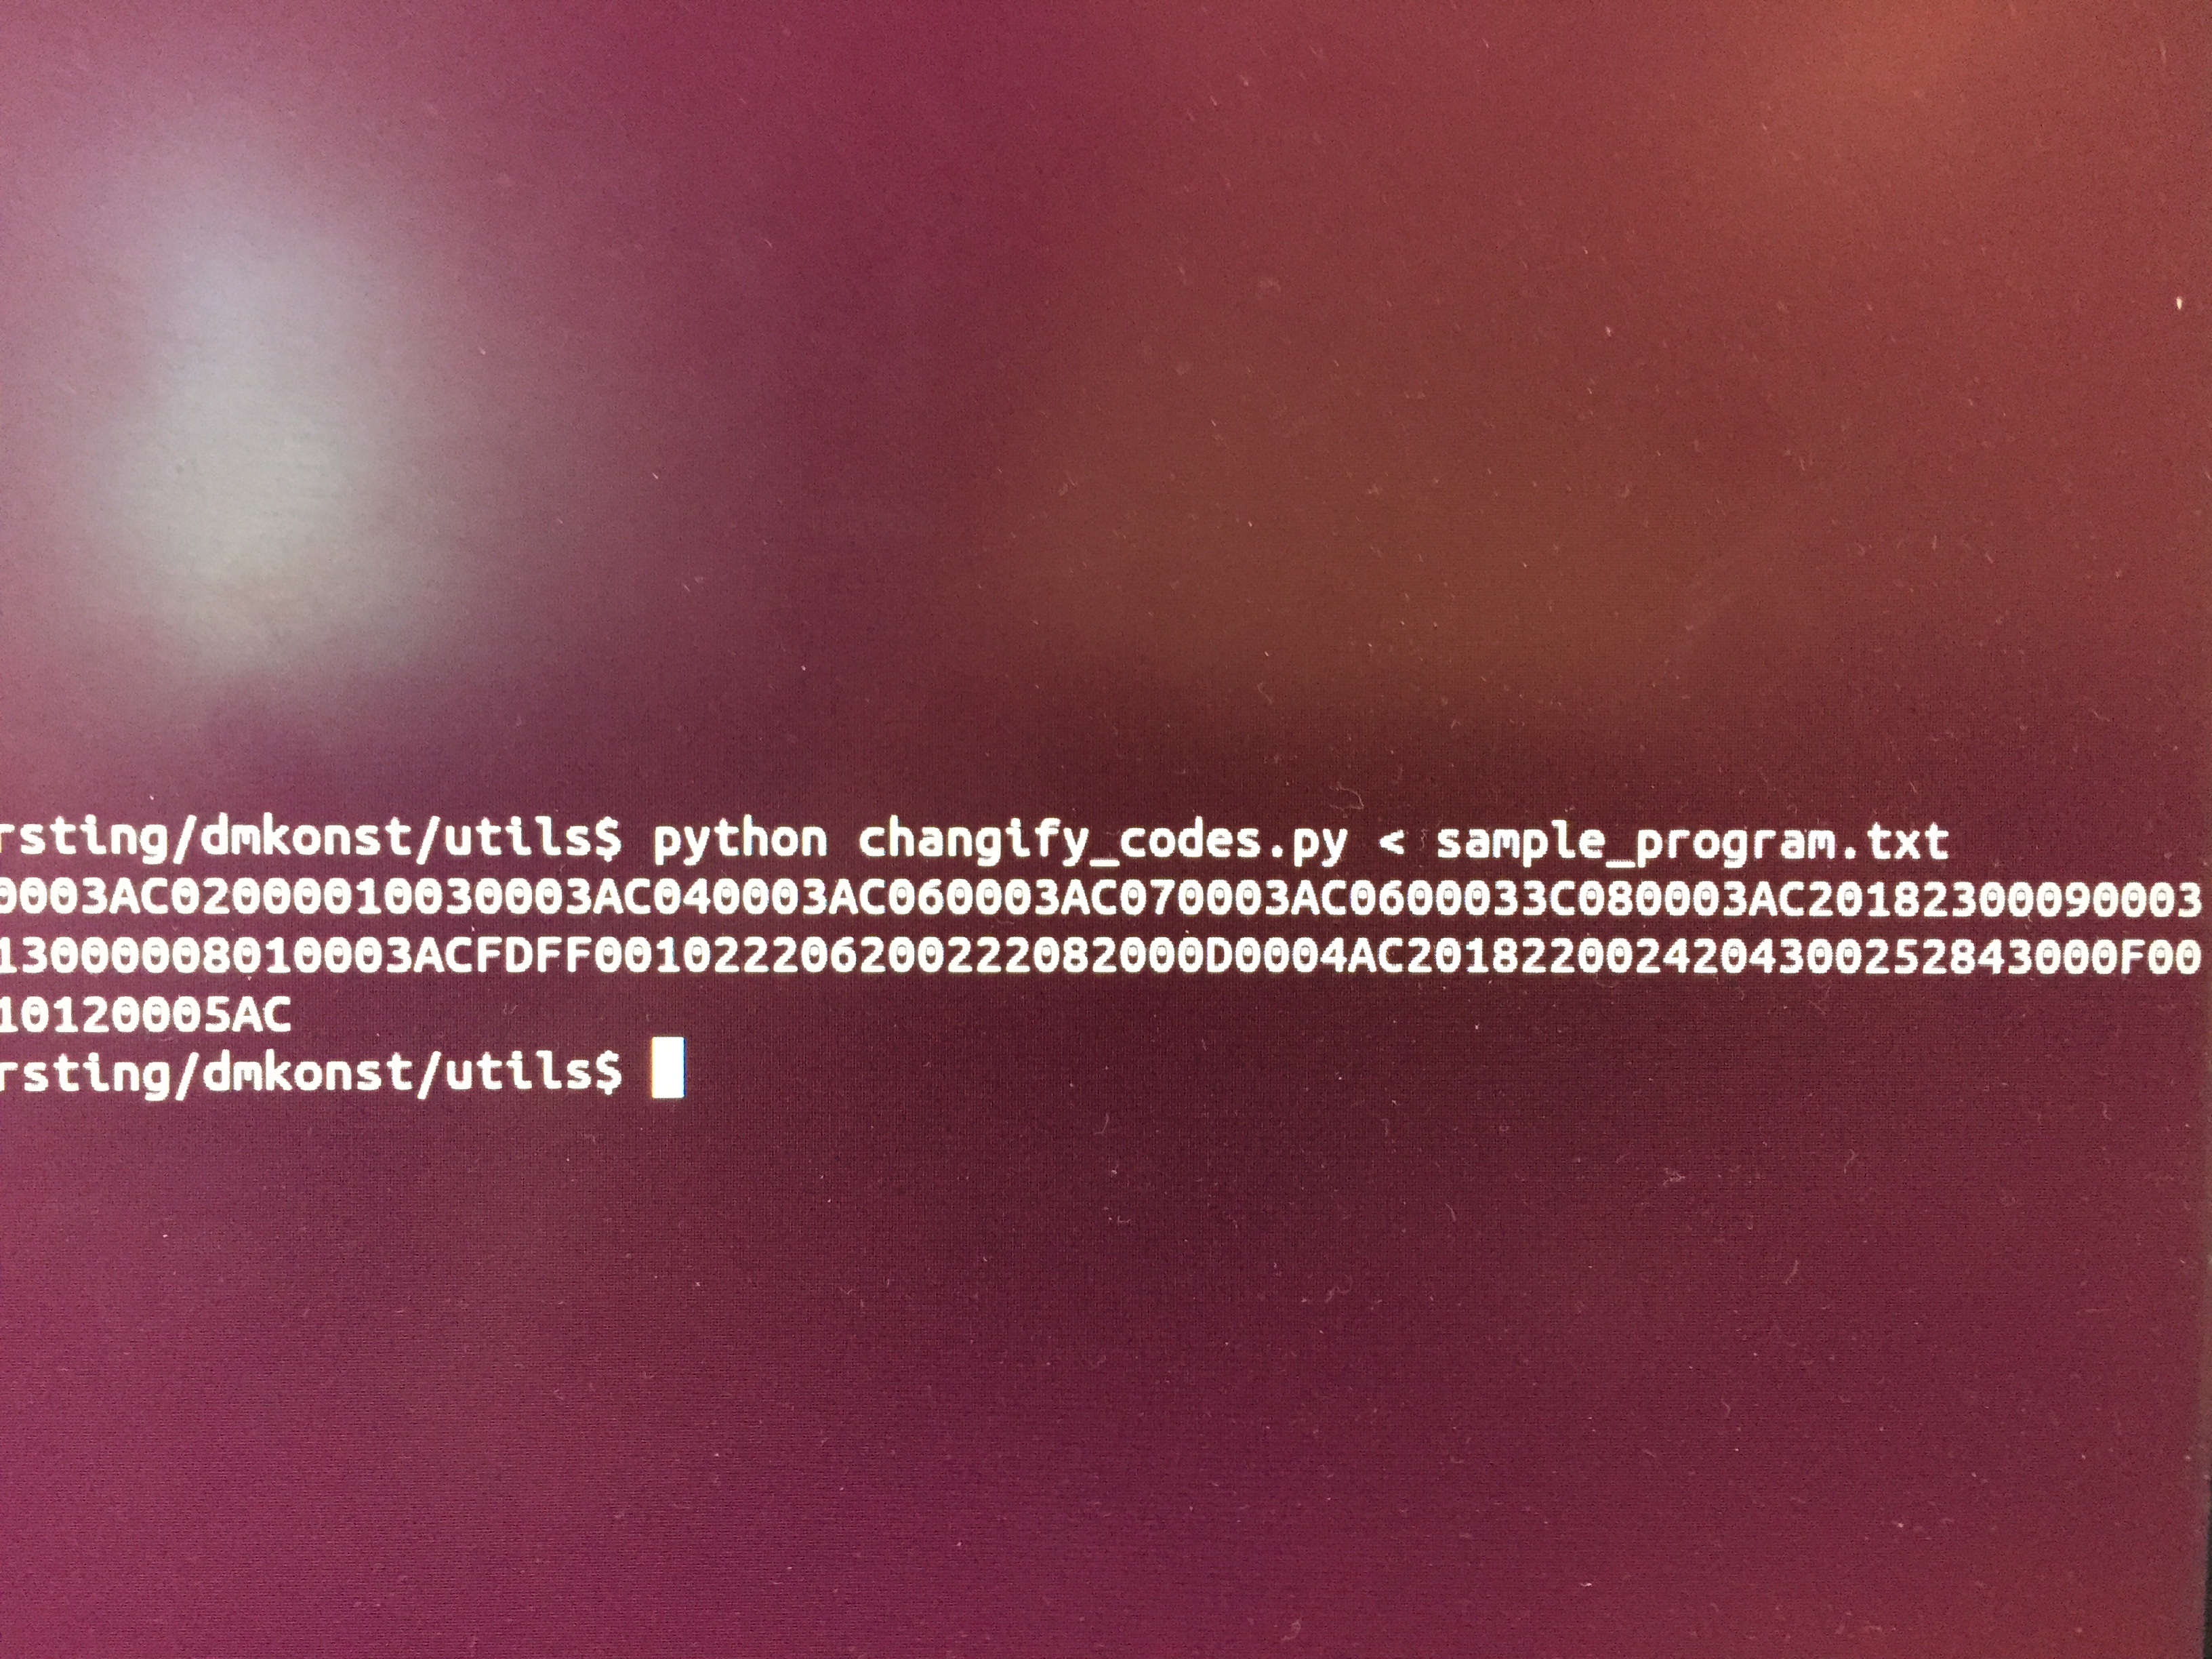
\includegraphics[width=0.4\textwidth]{assets/testing_on_fpga/change_endianness.JPG}
        }%
        \subfigure[Upload program to FPGA]{%
            \label{fig:program_upload_fpga}
            \includegraphics[width=0.4\textwidth]{assets/testing_on_fpga/upload_program_to_fpga.JPG}
        }\\ %%  ------- End of the second row ----------------------%
        \subfigure[Run program on FPGA]{%
            \label{fig:run_on_fpga}
            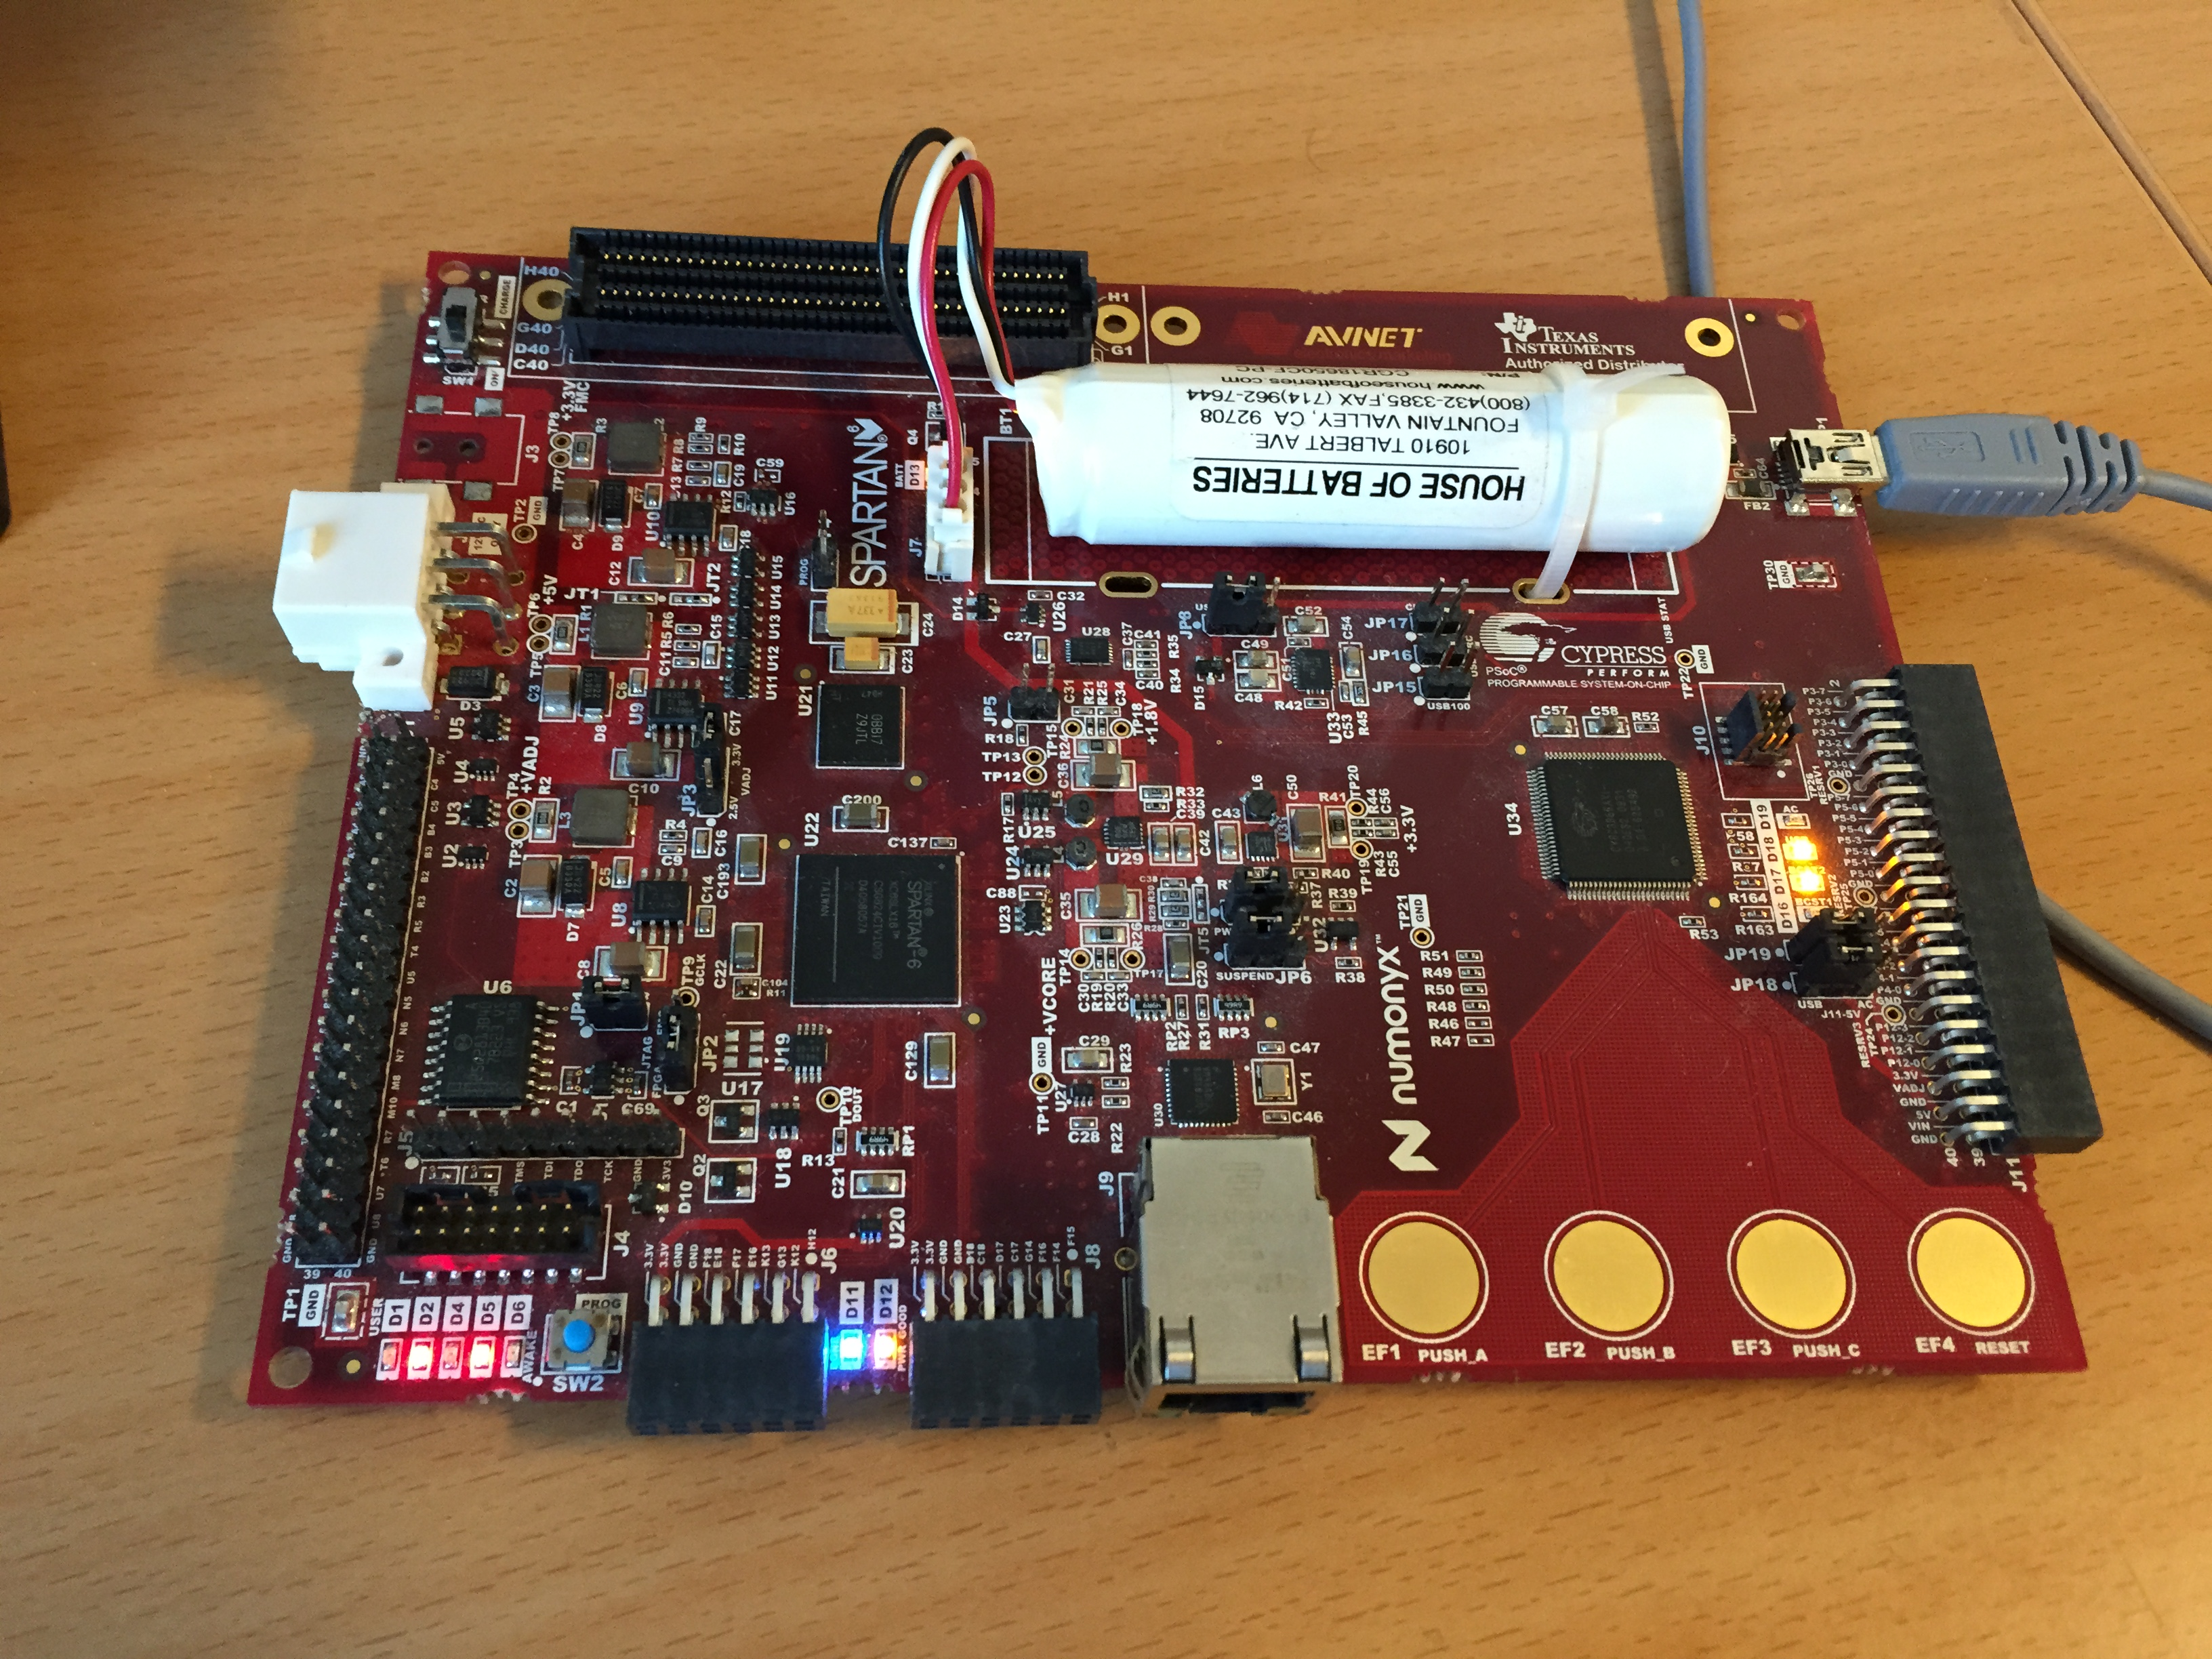
\includegraphics[width=0.4\textwidth]{assets/testing_on_fpga/run_on_fpga.JPG}
        }%
        \subfigure[Read data from FPGA]{%
            \label{fig:data_read_fpga}
            \includegraphics[width=0.4\textwidth]{assets/testing_on_fpga/data_read_from_fpga.JPG}
        }%
    \end{center}
    \caption{%
    Testing design on the FPGA in six simple steps.
    }%
    \label{fig:testing_on_fpga}
\end{figure}
